\section*{Úvod}
\label{sec:intro}
\addcontentsline{toc}{section}{\nameref{sec:intro}}
(Zpracováno podle knihy \cite{quantum})

Na konci 19. století se vědci domnívali, že s výjimkou několika detailů jejich teorie dokázaly odpovědět na všechny otázky fyziky. Podle nich už na obzoru nebyly žádné velké objevy. Maxwellovy rovnice elektromagnetismu a Newtonovy pohybové zákony kreslily deterministický vesmír: částice mají určitou pozici a momentum; síly působící na částici, určují změnu její pozice a rychlosti v čase - vše je předurčeno.

Ale už v roce 1900, při řešení problému absolutně černého tělesa, objevil Max Planck kvanta - nedělitelné balíky světla, jejichž velikost (energie) závisí na frekvenci daného světla. I když si v té době Max Planck i většina ostatních fyziků myslela, že to je pouze matematický trik, který nemá žádné implikace ve fyzickém světě, byl to první krok vedoucí ke kvantové revoluci.

Albert Einstein věřil ve fyzickou existenci Planckových kvant a ve vlnově-korpusku\-lární dualitu světla, podle níž je světlo částicí a vlnou zároveň a chová se jako jedno nebo druhé podle způsobu našeho pozorování. Ve svém Annus mirabilis\footnote[1]{Zázračný rok, ve kterém Einstein vydal 4 revoluční vědecké články.} (1905) kvantově vysvětlil fotoefekt: když elektron získá dostatek energie absorbcí kvanta světla, je uvolněn z obalu atomu a následně může být vyzařován.

Francouzský aristokrat Louis de Broglie vzal myšlenku kvant z Planckovy práce ještě dál a teoretizoval o vlnově-korpuskulární dualitě všech částic, nejen světelných, ale také částic hmotných.

Kvantový model atomu se postupně vyvíjel od modelu Nielse Bohra s jedním kvantovým číslem, vyjadřujícím velikost oběžné dráhy elektronu. Arnold Sommerfeld postupně k tomuto modelu přidal 3 další kvantová čísla: jedno vyjadřující tvar eliptické oběžné dráhy elektronu, druhé (magnetické) vyjadřující orientaci oběžné dráhy v prostoru a poslední vyjadřující spin, vnitřní moment hybnosti částice.

Bylo zřejmé, že je potřeba vytvořit teorii, která by popisovala fenomény kvantového světa: kvantovou mechaniku.

Roku 1925 Werner Heisenberg objevil Maticovou kvantovou mechaniku. Maticová, protože využívá matic a vektorů. Matice jsou tabulky čísel (viz Obrázek \ref{fig:1}), jež v této teorii mohou vyjadřovat veličiny jako polohu a hybnost částice. Vektory jsou veličiny, které mají kromě velikosti i směr a dají se vyjádřit maticemi. V Maticové mechanice se používají k vyjádření stavu systému, např. částice. Jelikož rozměry matic se zvyšují exponenciálně s rostoucím počtem částic, je tato teorie nesmírně nepraktická k výpočtu vývoje jakéhokoli systému.

\begin{figure}[ht]
    \centering
    $\begin{pmatrix}
    1 & 0 & 1 \\
    0 & 1 & 0 \\
    1 & 0 & 1
    \end{pmatrix}
    $
    \caption{\label{fig:1}Matice o 3 řádcích a 3 sloupcích.}
\end{figure}

Pouze tři měsíce po vydání Heisenbergova článku o Maticové mechanice zkonstruoval rakouský fyzik Erwin Schrödinger svou proslulou vlnovou rovnici (Rovnice (\ref{eq:1})), která popisuje vývoj vlnové funkce. Stala se základem Schrödingerovy Vlnové mechaniky. Výpočty s vlnovou rovnicí jsou daleko jednodušší, a tak se od Maticové mechaniky odstoupilo.

\begin{equation}
    \bm{i\hbar \frac{\partial \Psi}{\partial t} = -\frac{\hbar^2}{2m}
    \frac{\partial^2 \Psi}{\partial x^2} + V \Psi}
    \label{eq:1}
\end{equation}

O rok později Schrödinger dokázal matematickou ekvivalenci Maticové a Vlnové mechaniky: jsou to dvě formy téže teorie - kvantové mechaniky.

Krátce poté Max Born předložil pravděpodobnostní interpretaci vlnové funkce, v níž druhá mocnina vlnové funkce vyjadřuje pravděpodobnostní distribuční funkci výsledku. Pro ilustraci vezměte v úvahu obrázek \ref{fig:2}. $\bm{\Psi}$ je vlnová funkce, která vyjadřuje stav systému, např. pozici elektronu. \textbf{P} je pravděpodobnostní distribuční funkce. Tato funkce vyjadřuje pravděpodobnost pro každý možný výsledek měření (každá možná pozice elektronu). $\bm{P(x_0,x_1)}$ je pravděpodobnost, že výsledek měření bude mezi $x_0$ a $x_1$. V našem případě je to pravděpodobnost, že elektron bude mít pozici mezi $x_0$ a $x_1$ a počítá se integrací pravděpodobnost\-ní funkce mezi hodnotami $x_0$ a $x_1$. Integrací $(\int_{x_0}^{x_1}|\Psi|^2\,dx)$ získáme obsah pod křivkou v daném rozsahu odpovídající hledané pravděpodobnosti. 


\clearpage

\begin{figure}[ht]
\centering
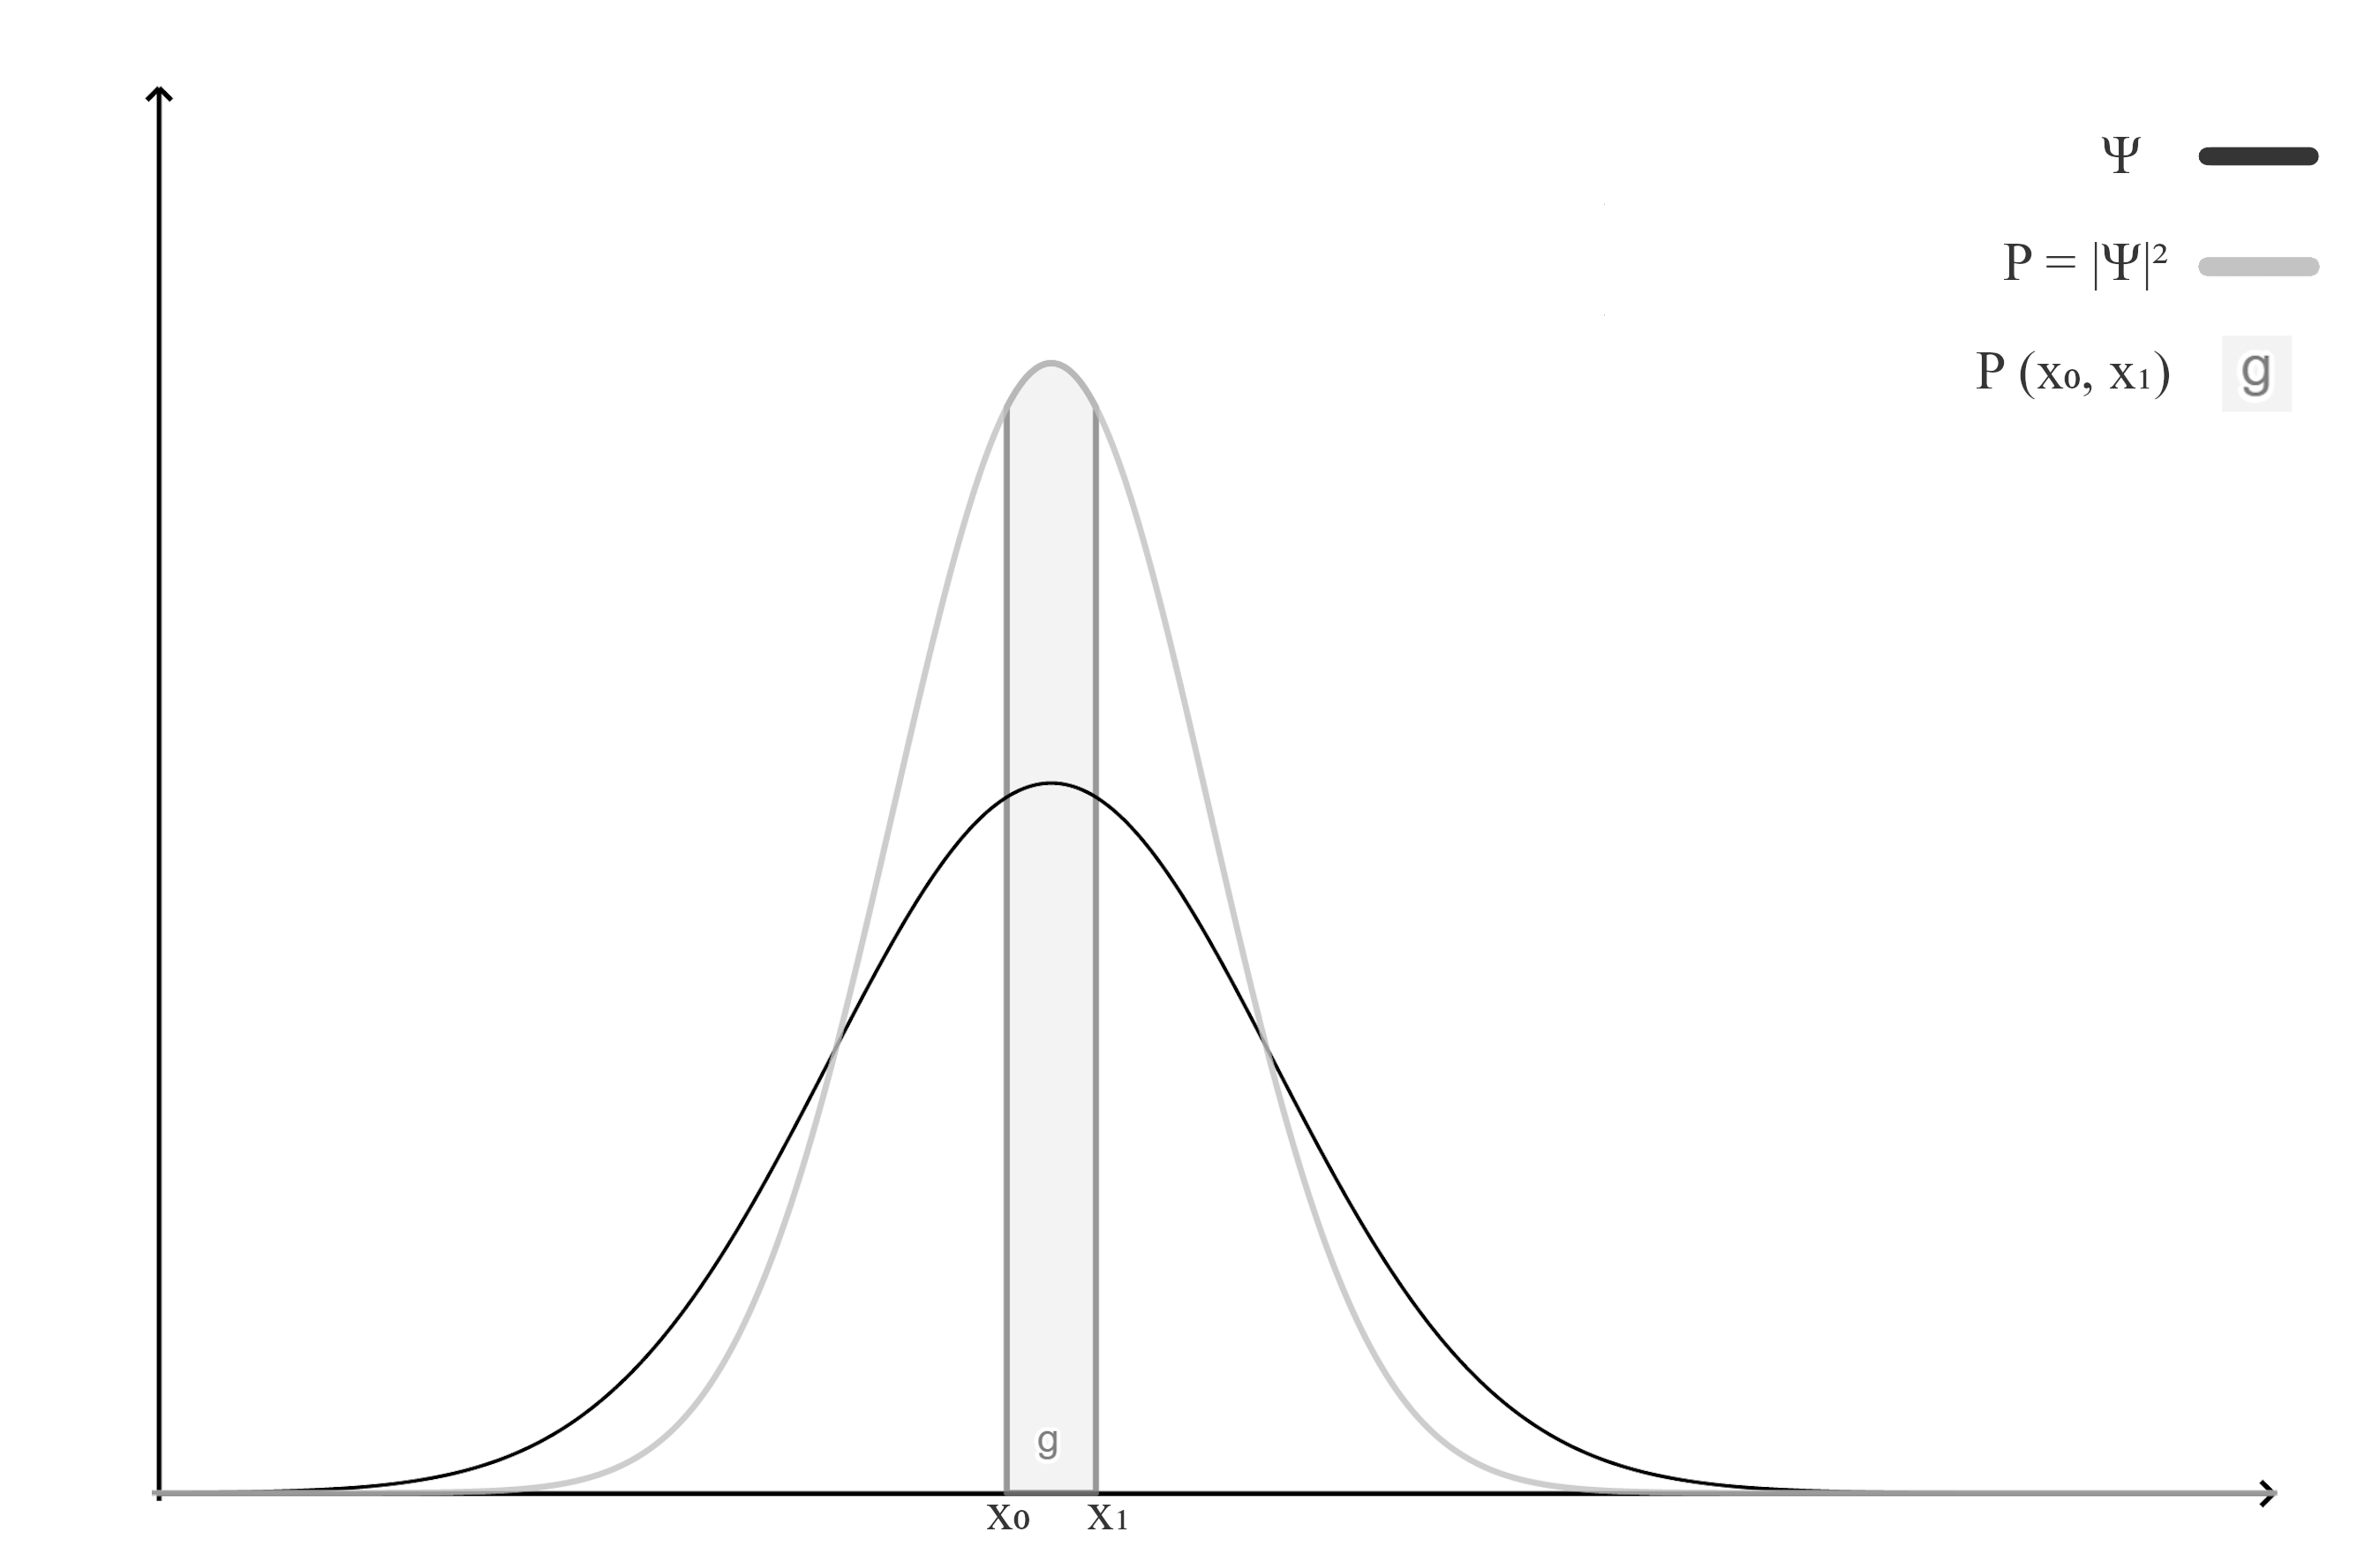
\includegraphics[width=300pt]{images/probability-function.png}
\caption{\label{fig:2}Vlnová funkce, pravděpodobnostní funkce a pravděpodobnost určitého výsledku.}
\end{figure}



Pravděpodobnostní interpretace se stala důležitou součástí dnešní kvantové mechaniky (Kodaňské interpretace), kterou společně definovali Bohr, Pauli a Heisenberg.

Kvantová mechanika změnila obraz vesmíru z deterministického a předurčeného na indeterministický a pravděpodobnostní. V kvantovém pravděpodobnostním vesmíru můžeme určit pouze pravděpodobnost daného výsledku. Jediný způsob, jak Clerk Maxwell a Ludwig Boltzmann mohli popsat vlastnosti plynu skládajícího se z nesčetného množství částic, bylo použitím pravděpodob\-nosti. Museli se spokojit se statistickým popisem. Tento nucený ústup ke statistické analýze byl způsoben neuskutečnitelností sledování pozice a rychlosti tolika částic. Pravděpodob\-nost byla důsledkem lidské nevědomosti. Naopak podle kvantové mechaniky je pravděpodobnost\-ní vyjádření kvantového světa fundamentální vlastností kvantového vesmíru.

Přestože se Albert Einstein na kvantové revoluci podílel, proměnil se v jejího nejhlasitějšího kritika. Uvědomoval si její užitečnost v atomových měřítcích, ale tvrdil, že \uv{Bůh ne{hraje v }kostky.} Byl přesvědčený, že kvantová mechanika není konečnou teoríí, že za ní musí být fundamentálnější deterministická teorie. Takovým teoriím se říká teorie se \uv{skrytými} parametry. Podle nich dokážeme určit jen pravděpodobnost výsledků, jelikož neznáme všechny parametry. Kdybychom znali \uv{skryté} parametry, dokázali bychom určit přesný výsledek měření.

V roce 1962 našel John Stewart Bell způsob, jak matematicky posoudit možnost teorie se skrytými parametry, která by replikovala výsledky kvantové mechaniky. Dnes se jí říká Bellova nerovnost. Tato nerovnost byla experimentálně porušena. Podle všeobecného mínění znamená porušení této nerovnosti nemožnost teorie se skrytými parametry. Porušení ale pouze znamená, že neexistuje teorie se skrytými parametry replikující kvantovou mechaniku, která by splňovala princip lokálního realismu a podmínku Statistické Nezávislosti.

Zde se budu věnovat teorii se skrytými parametry, která nesplňuje podmínku Statistické Nezávislosti. Takovou teorii nazval Bell Superdeterminismus. Statistická Nezávislost (viz Rovnice (\ref{eq:2})) znamená, že pravděpodobnostní distribuce skrytých parametrů ($\bm{P(\lambda)}$) se nezmění, vezmeme-li v potaz nastavení detektorů, \textbf{(a,b)}. Této podmínce se často říká podmín\-ka svobodné vůle nebo svobodné volby. 

Mým cílem je přehodnotit argumenty proti Superdeterminismu. V rozporu s všeobecným míněním se pokusím vysvětlit, že Superdeterminismus je cestou, která by mohla vyřešit mnoho problémů se současnými teoriemi a kterou bychom neměli ignorovat; je to cesta, kterou jsme se nevydali.

\begin{equation}
    \bm{P(\lambda|\bm{a},\bm{b}) = P(\lambda)} 
    \label{eq:2}
\end{equation}

